\chapter{Background Material}
\begin{comment}

\item RL Sutton book
\item deepmind lectures

\end{comment}

In order to correctly design the environments and implement reinforcement learning algorithms effectively, a certain amount of terminology needs to be understood. The first section of this chapter gives an overview of the basic terminology used within the reinforcement learning field. The second section discusses Markov decision processes, the mathematical framework used to formalize all reinforcement learning problems. In the final section of this chapter, the algorithms used in the rest of the dissertation are introduced. It is important to note this is only a brief overview of some basic concepts within reinforcement learning, for more detail please refer to Sutton and Barto's `Reinforcement Learning: An Introduction' \cite{Sutton:RLIntro01}.

\section{Basic Terminology}
Reinforcement learning is defined by the following:
\begin{quote}
A \textit{learning agent} interacts with its \textit{environment} by choosing \textit{actions} that affect the \textit{state} of the environment, and the eventual \textit{reward}. The agent seeks to develop a \textit{policy} that maximises reward by mapping states to the optimal actions.
\end{quote}
This definition has a few basic terms that need to be accurately described.

The \textit{learning agent} is the problem solver or operator itself, and the \textit{environment} is what this agent interacts with. In a game of chess, the player would be the agent, and the chess board would be the environment. An agent can have complete or incomplete control over its environment. For example, in chess the player can move its own pieces wherever it likes (within the constraints of the game - a bishop can only move diagonally and the king can only move one square at a time), but it cannot move the opponent's pieces, giving the agent incomplete control over the environment.

The \textit{actions} are simply that, the actions the agent can make at a given timestep. These actions affect the \textit{state} of the environment (positioning of pieces on a chess board). In this dissertation, as in many RL problems, we work with a special case where at every state the same set of actions can be performed - the action space is the same throughout the state space. 

Actions affect the state of the environment as well as the reward, both immediate and eventual. The \textit{reward} is a scalar value given at each timestep. In a game of chess, this could be 0 for each non-terminal move, 1 if the game results in a win, -1 if a loss and 0 for a stalemate. For a solution that requires reaching a goal state in the smallest amount of timesteps (such as golf), each timestep could provide a reward of -1 until the goal state is reached. A faster solution would then have a higher cumulative reward. Problems that don't have a terminal state are called continuous cases, and require slightly different treatment than cases with terminal states. In these cases a balance between valuing long term and short term reward must be found, and often require different mathematical treatment than cases with terminating states. Environments that terminate after a finite number of timesteps are called episodic cases, and are the type of cases that will be examined throughout this dissertation. 

A \textit{policy} is a function (either deterministic or stochastic) that maps states to actions in order to maximise cumulative reward. In tabular cases (those which have a finite set of discrete states and a finite set of discrete actions), the policy can often be represented as a matrix or dictionary, where each action within each state is given a probability for its selection. Often this policy is deterministic - the probabilities of all actions are 0 for a given state except for the action (or actions) that will bring the most reward, which would have a probability of 1 (or are given equal weights that sum to 1) - this is called a $greedy$ policy. Other policies are stochastic - even the actions considered less valuable have a non-zero chance of being chosen. These policies are often used because a learning algorithm needs to explore multiple paths to see if there is a possible reward resulting from an action. This is often termed `exploration vs exploitation' - policies often need to balance exploration - determining which algorithms are best, with exploitation - receiving the best possible reward. The most common type of stochastic policy is the $\varepsilon$-greedy function. $\varepsilon$-greedy functions act as greedy functions for the majority $1-\varepsilon$ of action choices, but for the remaining $\varepsilon$ all actions are chosen from with equal probability. Different policy types are used in different learning algorithms, as will be shown in section \ref{algorithms}.

\section{Markov Decision Processes}\label{MDP}
Markov decision processes (MDPs) are "a mathematically idealized form of the reinforcement learning problem for which precisely theoretical statements can be made".

By defining a problem using this framework, algorithms can be applied that are used throughout the reinforcement learning field. He we will re-frame some terms explained in the previous section under the MDP framework and provide their mathematical notation, as well as introduce some more concepts, before applying them to algorithms in the next section.

\begin{figure}[h]
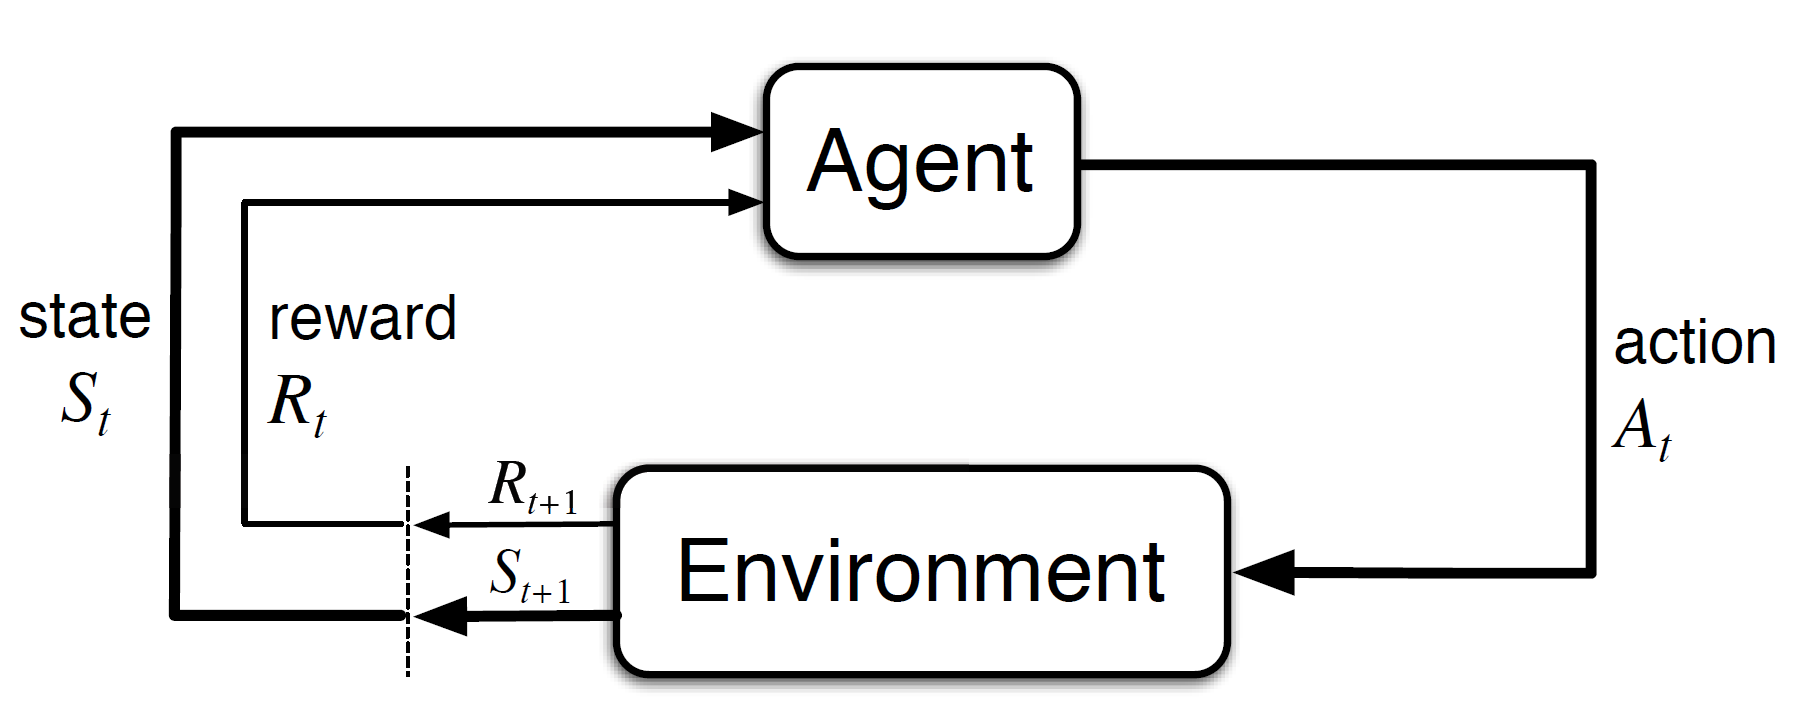
\includegraphics[width=\textwidth]{images/mdp}
\caption[Markov Decision Process]{graph displaying MDP taken from Sutton book}
\label{fig:mdp}
\end{figure}

MDPs frame an RL problem as seen in figure \ref{fig:mdp}. At each time step $t = 0\mathrm{,}1\mathrm{,}2\mathrm{,}3\mathrm{...}$ the agent receives information about the environment's state $S_{t}\in\mathscr{S}$, and selects an action $A_{t}\in\mathscr{A}$ based on the policy $\pi\left(A_t\mid S_t\right)$. At the next timestep, the agent receives a reward $R_{t+1}\in\mathscr{R}\subset\mathbb{R}$ and is in a new state $S_{t+1}$. This trajectory then continues: $S_0,A_0,R_1,S_1,A_1,R_2,S_2,A_2...$ until the episode terminates. 

The dynamics of a finite MDP (which has a finite set of states, actions, and rewards) is defined as a probability:
\begin{gather}
p(s',r\mid s,a) \doteq Pr\left\lbrace S_t=s',R_t=r \mid S_{t-1} = s, A_{t-1}=a\right\rbrace \\
\textnormal{where } p:\mathscr{S}\times\mathscr{R}\times\mathscr{S}\times\mathscr{A}\to\left[0,1\right] \nonumber \\
\textnormal{and } \sum_{s'\in\mathscr{S}}\sum_{r\in\mathscr{R}}p(s',r\mid s,a)=1, \textnormal{ for all }  s\in\mathscr{S},a\in\mathscr{A}\left(s\right) \nonumber
\end{gather}

These probabilities should completely characterise the dynamics of the environment in an ideal MDP. This means that states within the environment should have the \textit{Markov property}, which means the state must include all of the information needed to determine the next state and reward given the action selected - the history of all previous states can be thrown away and all important information must remain in the current state. An example of this is a toy helicopter. The state must include the current position and velocity of the helicopter in order to correctly determine the position of the helicopter in the next state. If the state included only position, it would either have to look to the previous state to calculate velocity, and therefore not be Markov (it cannot use history), or will not have enough information to determine the position of the next timestep. While useful from a theoretical standpoint to prove convergence of learning algorithms, in application of reinforcement learning, the Markov property can make solutions too computationally expensive, as will be discussed later on.

For episodic cases, the return $G_t$ is the sum of all rewards that have been given during the episode:
\begin{equation}
G_t \doteq R_{t+1}+R_{t+2}+R_{t+3}+...+R_T
\end{equation}

In many cases, immediate reward is considered more valuable than potential reward later on, so we can introduce a discount factor $\gamma\in\left(0,1\right]$:
\begin{equation}
G_t \doteq R_{t+1}+\gamma R_{t+2}+\gamma^2R_{t+3}+...+R_T = \sum^{\infty}_{k=0}\gamma^kR_{t+k+1}
\end{equation}
\begin{equation}
G_t = R_{t+1} + \gamma G_{t+1}
\end{equation}

A unified notation for returns for both episodic and continuing cases is:
\begin{equation}
G_t \doteq \sum^T_{k=t+1}\gamma^{k-t-1}R_k
\end{equation}

The expected return starting from a state $s$ and following a given policy $\pi$ is found using the \textit{value function}:

\begin{equation}
v_\pi\left(s\right) \doteq \mathbb{E}_\pi\left[G_t \mid S_t=s\right] = \mathbb{E}_\pi\left[\sum^{\infty}_{k=0}\gamma^kR_{t+k+1}\mid S_t=s\right]\textnormal{, for all } s\in\mathscr{S}
\end{equation}

and similarly, the expected return starting from a state $s$, choosing an action $a$ and then following policy $\pi$ is found using the \textit{action-value function}:

\begin{equation}
q_\pi\left(s,a\right) \doteq \mathbb{E}_\pi\left[G_t \mid S_t=s, A_t=a\right] = \mathbb{E}_\pi\left[\sum^{\infty}_{k=0}\gamma^kR_{t+k+1}\mid S_t=s, A_t=a\right]
\end{equation}
\begin{comment}
bellman eq definition
\begin{align}
v_\pi\left(s\right) &\doteq \mathbb{E}_\pi\left[G_t \mid S_t=s\right] \nonumber\\
&=\mathbb{E}_\pi\left[R_{t+1}+\gamma G_{t+1} \mid S_t=s\right] \nonumber\\
&=\sum_a\pi\left(a\mid s\right)\sum_{s'}\sum_{r}p\left(s',r\mid s,a\right)\left[r+\gamma\mathbb{E}_\pi\left[G_{t+1}\mid S_{t+1}=s'\right]\right] \nonumber\\
&=\sum_a\pi\left(a\mid s\right)\sum_{s',r}p\left(s',r\mid s,a\right)\left[r+\gamma v_\pi\left(s'\right)\right]\textnormal{, for all }s\in\mathscr{S}
\end{align}

optimal value function

\begin{equation}
v_*\left(s\right)\doteq\max_\pi v_\pi\left(s\right)
\end{equation}

optimal action value function
\begin{equation}
q_*\left(s,a\right)\doteq\max_\pi q_\pi\left(s,a\right) = \mathbb{E}\left[R_{t+1}+\gamma v_*\left(S_{t+1}\right)\mid S_t=s,A_t=a\right]
\end{equation}

bellman optimality equation
\begin{align}
v_*\left(s\right) &= \max_{a\in\mathscr{A}\left(s\right)}q_{\pi_*}\left(s,a\right) \nonumber\\
&=\max_a\mathbb{E}_{\pi_*}\left[G_t\mid S_t=s,A_t=a\right]\\
&=\max_a\mathbb{E}_{\pi_*}\left[R_{t+1}+\gamma G_{t+1}\mid S_t=s,A_t=a\right]\\
&=\max_a\mathbb{E}\left[R_{t+1}+\gamma v_*\left(S_{t+1}\right)\mid S_t=s,A_t=a\right]\\
&=\max_a\sum_{s',r}p\left(s',r\mid s,a\right)\left[r+\gamma v_*\left(s'\right)\right]
\end{align}

for q star
\begin{equation}
q_*\left(s,a\right)=\sum_{s',r}p\left(s',r\mid s,a\right)\left[r+\gamma\max_{a'}q_*\left(s',a'\right)\right]
\end{equation}
\end{comment}




\section{Algorithms}\label{algorithms}
Both algorithms discussed here use a concept called policy iteration. Policy iteration involves stepping through a process, using the data collected to update the value functions (or action-value functions), and then updating the policy so it is greedier to the newly calculated value function. More data is then collected under this policy, and as this policy will likely take a different path than the previous policy, it will receive different rewards and thus update the value function again. By repeating this process continuously the policy eventually converges to its optimal state. 
\begin{comment}
\begin{wrapfigure}{l}{.27\textwidth}
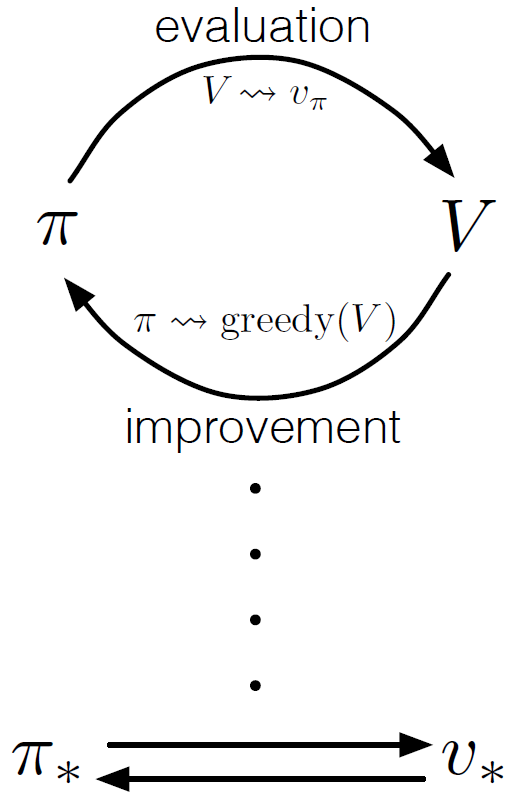
\includegraphics[width=.25\textwidth]{images/gpi}
\caption[Generalised policy iteration]{generalised policy iteration taken from sutton}
\end{wrapfigure}
\end{comment}
\begin{figure}[h]
\centering
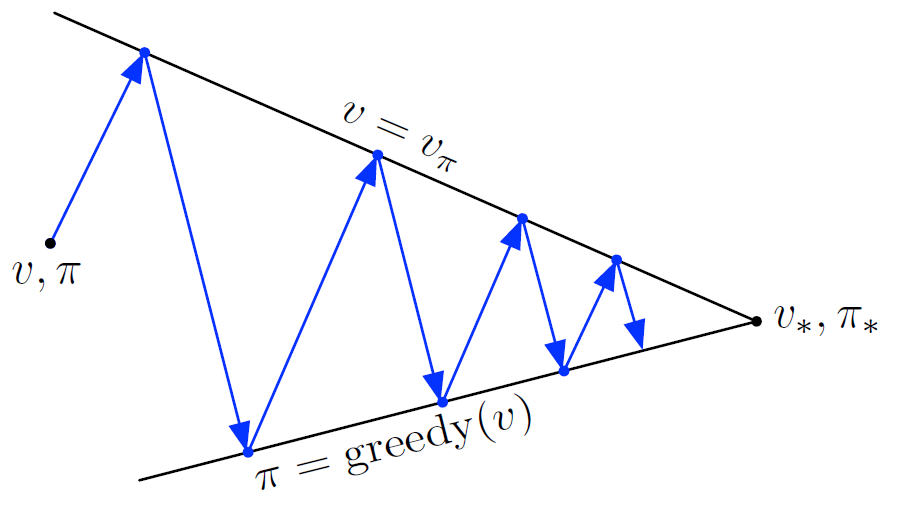
\includegraphics[width=.5\textwidth]{images/gpi2}
\caption[policy and value function convergence]{policy and value function convergence taken from sutton}
\end{figure}
\newpage
\subsection{Monte Carlo}

\begin{wrapfigure}{r}{.27\textwidth}
\vspace{-.6cm}
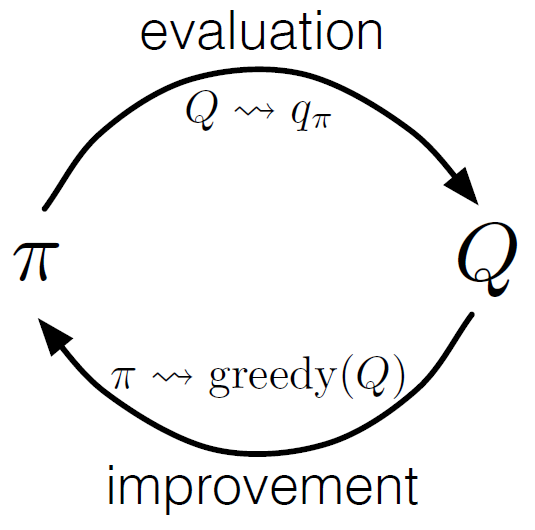
\includegraphics[width=.25\textwidth]{images/gpimc}
\caption[monte carlo policy iteration]{monte carlo policy iteration taken from sutton}
\label{fig:gpimc}
\end{wrapfigure}

\begin{figure}[h]
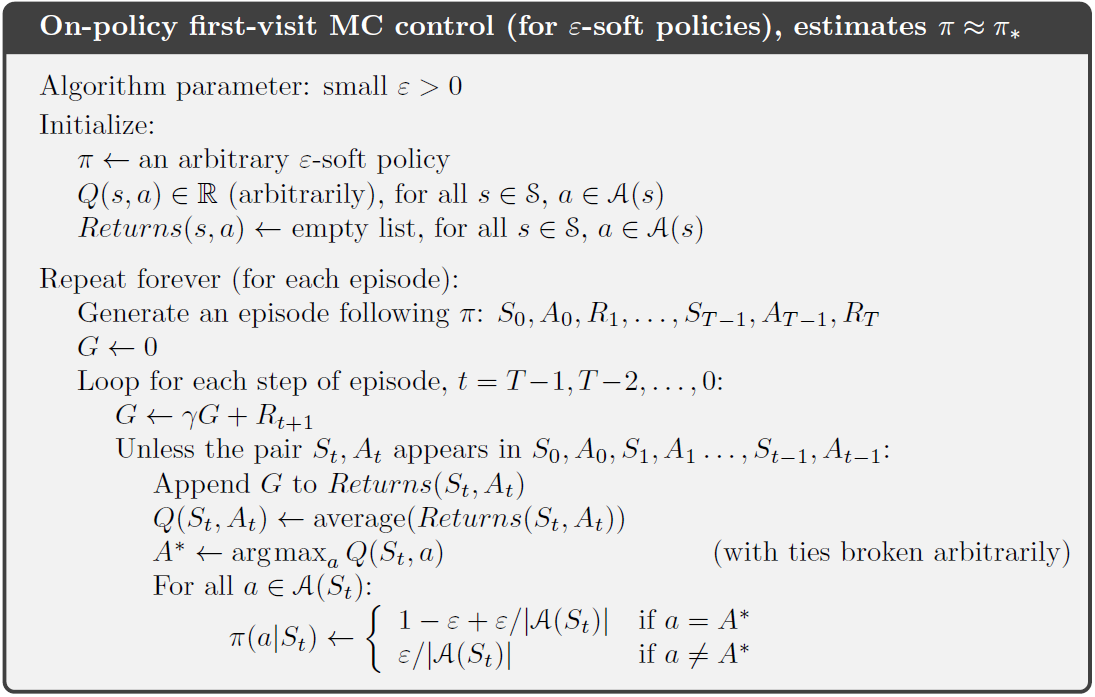
\includegraphics[width=\textwidth]{images/onpolicymc}
\caption[mc algorithm pseudocode]{mc algo pseudocode taken from sutton}
\label{fig:mcsuttonpseudo}
\end{figure}

Monte Carlo methods iterate only at the end of each episode as opposed to every step. This method works by gathering the full return of an episode, and updating the value function of each state that occurred within the episode to reflect this return. Note however it only updates each state once on the first visit, so if a state is visited more than once in an episode, the return is only counted the first time. To ensure all states are explored while maintaining a suitable level of exploitation, Monte Carlo algorithms implement an $\varepsilon$-soft policy, so that the optimal action is taken with a probability of $1-\varepsilon+\varepsilon/|\mathscr{A}\left(S_t\right)|$, where $|\mathscr{A}\left(S_t\right)|$ is the total number of actions, and all other actions are taken with a probability of $|\mathscr{A}\left(S_t\right)|$.
\begin{comment}

"A fourth advantage of Monte Carlo methods, which we discuss later in the book, is
that they may be less harmed by violations of the Markov property. This is because they
do not update their value estimates on the basis of the value estimates of successor states.
In other words, it is because they do not bootstrap." summary ch 5.10 ~\cite{Sutton:RLIntro01}
\end{comment}

\subsection{Q-Learning}

Unlike Monte Carlo, Q-Learning is off-policy, which means the algorithm generally has two policies: one that is used to gather the reward, which is normally a pure greedy function, and another separate policy to gather data, which  explores much more than a typical $\varepsilon$-greedy function. This means the algorithm can effectively explore and exploit simultaneously. Also unlike MC algorithms, Q-learning updates the state-action values after every step, not just at the end of an episode, using the function:

\begin{equation}
Q\left(S_t,A_t\right) \leftarrow \left(1-\alpha\right)Q\left(S_t,A_t\right) + \alpha\left[R_{t+1}+\gamma \max_aQ\left(S_{t+1},a\right)\right]
\end{equation}

\begin{figure}[h]
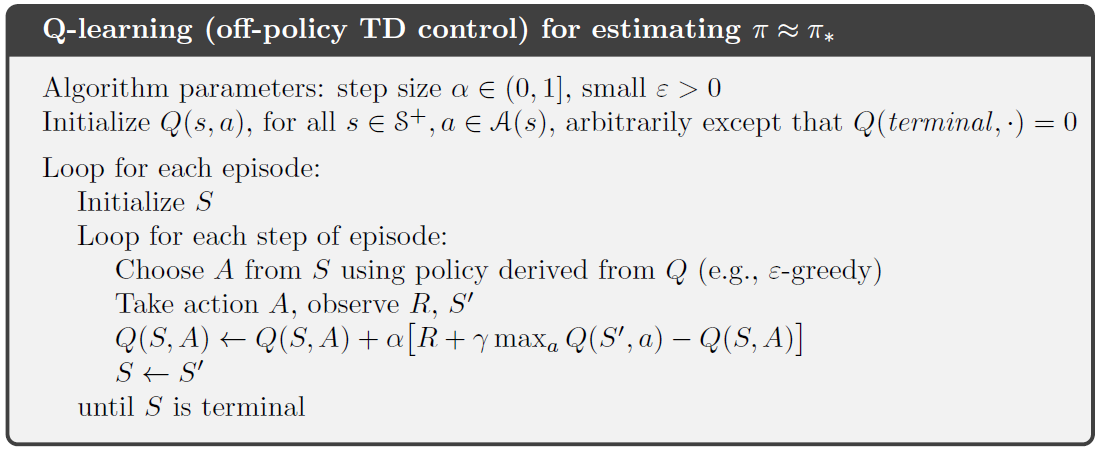
\includegraphics[width=\textwidth]{images/Q-learning}
\caption[Q-learning pseudocode]{Q-learning pseudocode taken from sutton}
\end{figure}
